\chapter{Management}


% Gestion de projet (méthode agiles ?, rythme des contacts avec votre tuteur, un diagramme de Gantt, ...)

An agile like method has been used during this project. The project has been devided into three major parts, corresponding to 
\begin{inparaenum}[1)] 
	\item the first module, 
	\item the second module, and 
	\item the report and the documentation writting. 
\end{inparaenum} 
The gantt diagrams of each part are displayed on the \vref{fig:diagram:gantt:part1,fig:diagram:gantt:part2,fig:diagram:gantt:part3}. 

Each part has been divided into multiple little tasks to be implemented one by one. Regular meetings with the supervisor were planned and as soon as a task has been finished. The meeting's goals were to present the current status of the cuurent task, and to discust about the next task to be done if the last one was finished. Meetings with the supervisor were less regular during the last month because of the resumption university courses. Meetings with the head of the \gls{IT} department where planned, usually at the end of the month, in order to show the project progres. 


\begin{figure}[H]
	\centering
	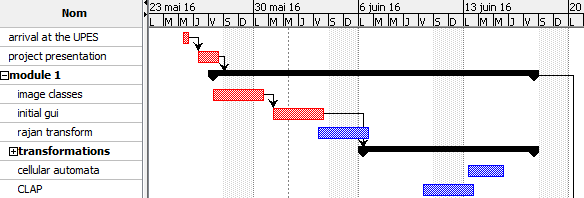
\includegraphics[width=0.8\textwidth]{images/gantt/gantt_part_1}
	\caption{Gantt diagram - part 1, first module}
	\label{fig:diagram:gantt:part1}
\end{figure}


\begin{figure}[H]
	\centering
	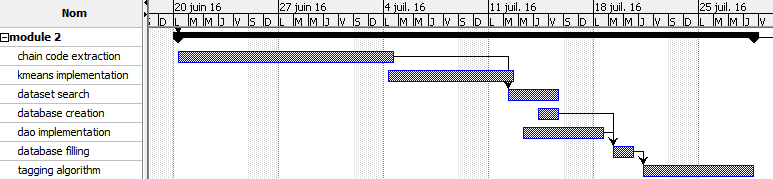
\includegraphics[width=1\textwidth]{images/gantt/gantt_part_2}
	\caption{Gantt diagram - part 2, second module}
	\label{fig:diagram:gantt:part2}
\end{figure}


\begin{figure}[H]
	\centering
	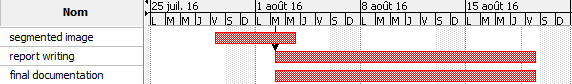
\includegraphics[width=0.8\textwidth]{images/gantt/gantt_part_3}
	\caption{Gantt diagram - part 3, documentation and writing}
	\label{fig:diagram:gantt:part3}
\end{figure}
	




